\documentclass[tikz,border=4pt]{standalone}
% Shared art direction for the "phones" post, after Vagrancy's region art
% (vagrancy/analysis/art/regions.py and data/palette.json "art"): flat fills,
% plum ink lines, a mustard sky, peach and sage. Every colour below is copied
% from that palette so the post and the game look like one hand drew them.
%
% The scenes share a horizon at y=2.6 and the same sky band, so consecutive
% figures read as one continuous walk down the page.
\usetikzlibrary{arrows.meta,calc,decorations.pathmorphing}
\definecolor{ink}{HTML}{3B2A3F}
\definecolor{sky}{HTML}{E9C46A}
\definecolor{skylight}{HTML}{F2DC98}
\definecolor{cloud}{HTML}{F6E7B8}
\definecolor{peach}{HTML}{EBA77C}
\definecolor{peachdark}{HTML}{D98B5C}
\definecolor{cream}{HTML}{F3E6C4}
\definecolor{sage}{HTML}{9DB58A}
\definecolor{sagedark}{HTML}{6F8F66}
\definecolor{olive}{HTML}{B9B566}
\definecolor{teal}{HTML}{79ADA4}
\definecolor{tealdark}{HTML}{4F8580}
\definecolor{slate}{HTML}{6E8494}
\definecolor{stone}{HTML}{C9B79C}
\definecolor{wood}{HTML}{A9774E}
\definecolor{gold}{HTML}{E3B04B}
\definecolor{shadow}{HTML}{5B4A63}
\tikzset{
  ln/.style={draw=ink, line width=0.9pt, line join=round},
  thinln/.style={draw=ink, line width=0.6pt, line join=round},
  lab/.style={font=\sffamily\scriptsize, text=ink, align=center},
  tag/.style={font=\sffamily\scriptsize\bfseries, text=ink, align=center},
}
% A walking figure. #1 x, #2 y, #3 body colour, #4 head tilt in degrees
% (0 upright, negative looking down at a phone).
\newcommand{\walker}[4]{%
  \begin{scope}[shift={(#1,#2)}]
    \filldraw[fill=#3, ln] (-0.13,0) rectangle (0.13,0.52);
    \draw[ln] (-0.09,0) -- (-0.14,-0.28);
    \draw[ln] (0.09,0) -- (0.17,-0.26);
    \begin{scope}[rotate around={#4:(0,0.52)}]
      \filldraw[fill=cream, ln] (0,0.66) circle (0.14);
    \end{scope}
  \end{scope}}

\begin{document}
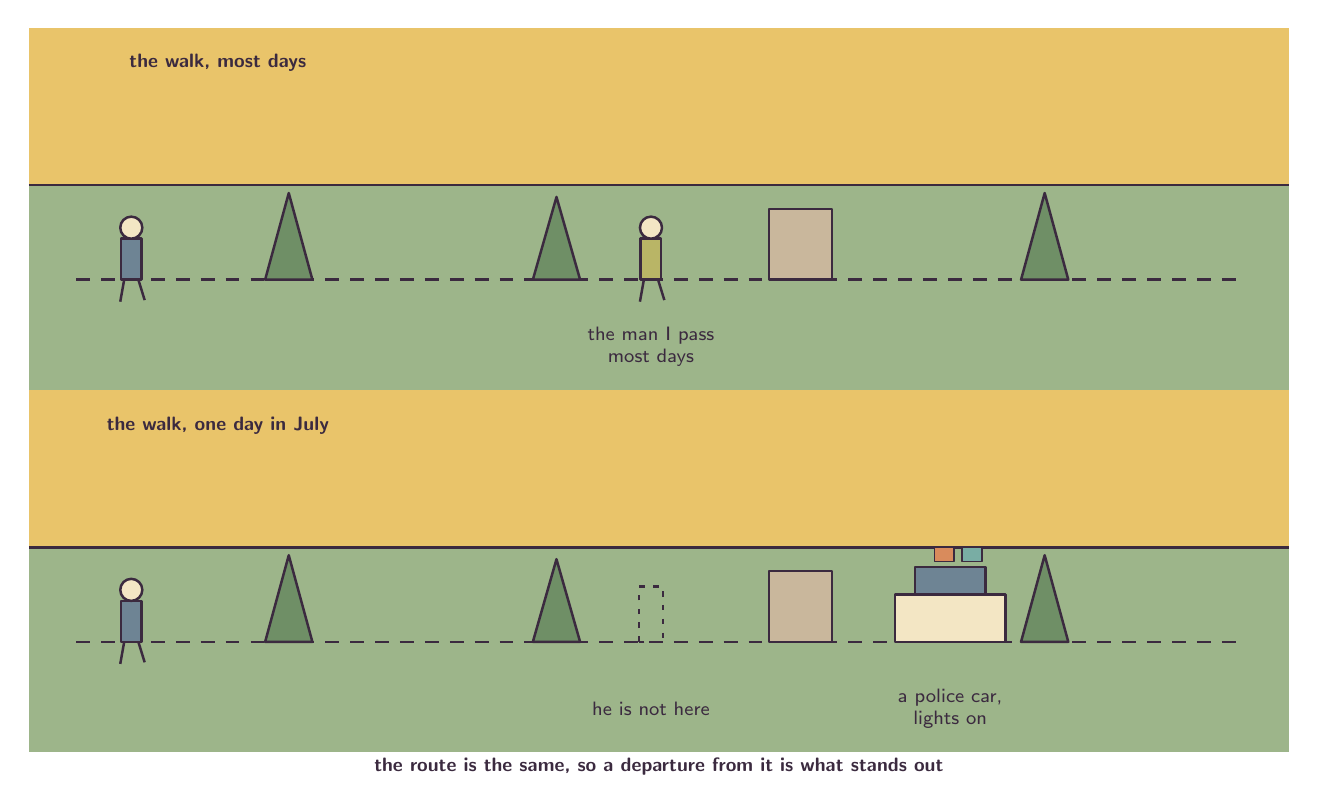
\begin{tikzpicture}[font=\sffamily]
  % Two passes of the SAME route. The scenery is identical between them, which
  % is the point: only then does a departure read as a departure.
  \foreach \p/\dy/\title in {0/0/{the walk, most days}, 1/-4.6/{the walk, one day in July}}{
    \begin{scope}[shift={(0,\dy)}]
      \fill[sky] (0,2.6) rectangle (16,4.6);
      \fill[sage] (0,0) rectangle (16,2.6);
      \draw[ln] (0,2.6) -- (16,2.6);
      \draw[ln, dash pattern=on 5pt off 4pt] (0.6,1.4) -- (15.4,1.4);
      \node[tag] at (2.4,4.15) {\title};
      % Fixed scenery: identical in both panels.
      \filldraw[fill=sagedark, ln] (3.0,1.4) -- (3.3,2.5) -- (3.6,1.4) -- cycle;
      \filldraw[fill=sagedark, ln] (6.4,1.4) -- (6.7,2.45) -- (7.0,1.4) -- cycle;
      \filldraw[fill=stone, ln] (9.4,1.4) rectangle (10.2,2.3);
      \filldraw[fill=sagedark, ln] (12.6,1.4) -- (12.9,2.5) -- (13.2,1.4) -- cycle;
      \walker{1.3}{1.4}{slate}{0}
    \end{scope}}
  % Top panel: the man who is always there.
  \walker{7.9}{1.4}{olive}{0}
  \node[lab, text width=2.8cm] at (7.9,0.55) {the man I pass\\most days};
  % Bottom panel: he is absent, and something else is not.
  \draw[ln, dash pattern=on 2pt off 3pt] (7.75,-3.2) rectangle (8.05,-2.5);
  \node[lab, text width=2.6cm] at (7.9,-4.05) {he is not here};
  \filldraw[fill=cream, ln] (11.0,-3.2) rectangle (12.4,-2.6);
  \filldraw[fill=slate, ln] (11.25,-2.6) rectangle (12.15,-2.25);
  \filldraw[fill=peachdark, thinln] (11.5,-2.18) rectangle (11.75,-2.0);
  \filldraw[fill=teal, thinln] (11.85,-2.18) rectangle (12.1,-2.0);
  \node[lab, text width=3cm] at (11.7,-4.05) {a police car,\\lights on};
  \node[tag, text width=13cm] at (8.0,-4.78) {the route is the same, so a departure from it is what stands out};
\end{tikzpicture}
\end{document}
